\newcommand{\letitle}{Sur la vérification de preuve et la preuve automatique d'appartenance d'un mot à une grammaire.}
\newcommand{\leauthor}{Ulysse Durand}

\documentclass[a4paper,12pt]{article}
\usepackage{tikzit}

\usepackage[utf8]{inputenc}
\usepackage{amssymb}
\usepackage{amsmath}
\usepackage{xcolor}
\usepackage{enumitem}
\usepackage[margin=3cm]{geometry}
\usepackage{bbold}
\usepackage[xcolor,leftbars]{changebar}

\setcounter{secnumdepth}{1}
\newenvironment{myindentpar}
 {\begin{list}{}
         {\setlength{\leftmargin}{1em}}
         \item[]
 }
 { \end{list}}

\definecolor{DarkBlue}{RGB}{0,16,80}
\newcommand{\norm}[1]{\lvert #1 \rvert}
\newsavebox{\mybox}
\newlength{\mydepth}
\newlength{\myheight}
\newenvironment{answer}
{\par\begin{lrbox}{\mybox}\quad\begin{minipage}{\linewidth}\color{black}\setlength{\parskip}{10pt plus 1pt minus 1pt}\vspace*{-.7\baselineskip}}
{\end{minipage}\end{lrbox}
\settodepth{\mydepth}{\usebox{\mybox}}
\settoheight{\myheight}{\usebox{\mybox}}
\addtolength{\myheight}{\mydepth}
\noindent\makebox[0pt]{
  \color{gray}\hspace{-0pt}\rule[-\mydepth]{1pt}{\myheight}}
  \usebox{\mybox}
  }

\usepackage{hyperref}
\setlength{\parskip}{0.15cm}
\hypersetup{
    colorlinks=truem,
    linkcolor=black,
    filecolor=red,
    urlcolor=blue
}

\urlstyle{same}

\everymath{\displaystyle}
\title{\letitle}
\author{\leauthor}
\date{}
\begin{document}
    
\maketitle
\tableofcontents

\section{Définitions}

\subsection{Les grammaires formelles}

Une grammaire formelle est un quadruplet $G = (T,N_t,S,D)$ où :

\begin{itemize}
\item $T$ est l'alphabet des terminaux
\item $N_t$ est l'alphabet des non terminaux
\item $S \in N_t$ est l'axiome

Notons $\Sigma := N_t \cup T0$
\item $D \subset (\Sigma ^ \star )^2$, est l'ensemble des règles de dérivation.
\end{itemize}
Pour $(a,b) \in D$, soit $\overset{(a,b)}{\rightarrow}$ la relation binaire définie sur $\Sigma^\star$ par
\begin{equation*}
\forall m,m' \in \Sigma^\star, m \overset{(a,b)}{\rightarrow} m' \iff \exists u,v \in \Sigma^\star / m = uav \text{ et } m' = ubv
\end{equation*}
On note $\rightarrow := \bigcup_{d \in D} \overset{d}{\rightarrow}$ et on note $\overset{*}{\rightarrow}$ la cloture transitive et réflexive de $\rightarrow$.\\
Pour $x \in (\Sigma)^\star$, notons\\
$\delta(x) := \{y \in (\Sigma)^\star / x \overset{*}{\rightarrow} y\}$\\
$\eta(x) := \delta(x) \cap T^\star$\\
$\norm{x}_l := \norm{\{i \in \mathbb{N} \mid x_i = l \}}$ est le nombre d'occurences de la lettre $l$ dans x.

Alors le langage de la grammaire formelle  G est le suivant :
\begin{equation*}\mathcal{L} (G) := \eta(S)\end{equation*}

Nous allons supposer que $N_t$ est dénombrable et $T$ est fini.

En OCaml :
{\color{DarkBlue}\begin{verbatim}
type 'e caractere = T of 'e | Nt of int

type 'a regle = ('a array) * ('a array)

type 'e fg = {
  terminaux : ('e caractere) array ;
  nonterminaux : ('e caractere) array ;
  axiome : 'e caractere ;
  reglesf : ('e caractere) regle array
} 
\end{verbatim}}
\subsection{Les grammaires non contextuelle}

\textbf{  Définition : } Une grammaire non contextuelle est une grammaire $G = (T,N_t,S,D)$ telle que :
\begin{equation*} \forall (a,b) \in D, a \in N_t  \end{equation*}
(Nous identifions les mots de longueur 1 et les lettres)

{\color{DarkBlue}\begin{verbatim}
type 'a reglecf = int * ('a array)

type 'e cfg = {
  terminaux : ('e caractere) array ;
  nonterminaux : ('e caractere) array ;
  axiome : 'e caractere ;
  reglescf : ('e caractere) reglecf array
}
\end{verbatim}}

\textbf{ Exemple : } la grammaire non contextuelle des expressions arithmétiques suffixes.
\begin{align*}
D = &\{(\underline{ S },\underline{ SS+ })_1,(\underline{ S },\underline{ SS* })_2,(\underline{ S },\underline{ "N" })_3\}\\
\cup&\{(\underline{ N },\underline{ C })_4 | (\underline{ N },\underline{ NC })_5\}\\
\cup&\{(\underline{ C },\underline{ 0 })_6 | (\underline{ C },\underline{  1 })_7\}
\end{align*}
(les indices ci-dessus correspondent à une énumération des règles de dérivation, par exemple, $D_5 = (\underline{ N },\underline{ NC })$)

\subsection{Fôret de dérivation}

Ici, $G = (T,N_t,S,D)$ est une grammaire non contextuelle.

Une forêt est une liste d'arbres
{\color{DarkBlue}\begin{verbatim}
type 'a arbre = 'a * 'a foret 
and 'a foret = F of 'a arbre list
\end{verbatim}}


Une preuve qu'un mot appartient à $\eta(m)$ peut être donnée par une forêt de dérivation de $m$:

\begin{answer} 
Si $m$ est le mot vide, il s'agit de la forêt vide.

Sinon, soit $n = \norm{m}$,\\
\begin{answer} 
    Si $n=1$ et $m_0 \in T$,il s'agit d'un seul arbre où la racine est $m$ et la sous forêt est la forêt de dérivation d'un $b$ tel que $(m,b) \in D$.

    Si $n=1$ et $m_0 \in N_t$, il s'agit de l'arbre de racine m et de sous forêt vide.

    Si $n>1$, il s'agit de la liste des arbres $[f_1, \dots, f_n]$ où $\forall i \in [1,n], f_i$ est un arbre de dérivation de la lettre $m_i$.
\end{answer}
\end{answer}

D'où la fonction OCaml suivante :

{\color{DarkBlue}\begin{verbatim}
let rec test_foret_deriv foret mot regles =
  let n = List.length mot in
  if n = 0 then foret = F [] else
  match foret with
      |(F sousarbres) ->
          if (List.length sousarbres) <> n then false else
          List.for_all2
          (fun arb lettre ->
              test_arbre_deriv arb regles
          )
          sousarbres
          mot
and test_arbre_deriv arb regles =
  let (lettre,sousforet) = arb in
  match lettre with
      |T x -> arb = (T x,F [])
      |Nt i ->
          let nouveaumot = lisracines sousforet in
          (List.mem (i,nouveaumot) regles)&&
          (test_foret_deriv sousforet nouveaumot regles)
\end{verbatim}}

L'ensemble des forêts de dérivation de $m$ est noté $\mathcal{F}(m)$.\\
Le parcours infixe des feuilles d'une forêt de dérivation de $x$ donne un mot de $\eta(x)$.
Un exemple sera donnée dans le cas d'une grammaire non contextuelle.\\
Pour $a \in \mathcal{F}(x)$, on note $\mathcal{I}(a)$ le parcours infixe des feuilles de $a$. 

\subsection{Exemple de preuve}

Une preuve que \underline{ "10""11"+"0"* } $\in \mathcal{L}(G)$ :\\
Lemme 1 : \underline{ "10" } $\in \eta(S)$

    En effet, $\underline{ S }\rightarrow_3 \underline{ "N" } \rightarrow_5 \underline{ "NC" } \rightarrow_6 \underline{ "N0" } \rightarrow_4 \underline{ "C0" } \rightarrow_7 \underline{ "10" }$


L'abre de dérivation fait aussi office de preuve, bien plus concise :
   
\begin{tikzpicture}[level distance=20pt]
    \node {S}
child { node {"} }
child {
    node {N}
    child {
        node {N}
        child {
            node {C}
            child {
                node {1}
            }
        }
    }
    child {
        node {C}
        child {
            node {0}
        }
    }
}
child { node {"} }

    ;
\end{tikzpicture}
    

Lemme 2 : \underline{ "11" } $\in \eta(S)$
Preuve avec l'arbre suivant
 
\begin{tikzpicture}[level distance=20pt]
    \node {S}
child { node {"} }
child {
    node {N}
    child {
        node {N}
        child {
            node {C}
            child {
                node {1}
            }
        }
    }
    child {
        node {C}
        child {
            node {1}
        }
    }
}
child { node {"} }

    ;
\end{tikzpicture}
    

On peut alors, en combinant les deux arbres précédants, prouver que \underline{ "10""11"+ } $\in \eta(S)$ :
 
\begin{tikzpicture}[level distance=20pt]
    \tikzstyle{level 1}=[sibling distance=30mm]
\tikzstyle{level 2}=[sibling distance=10mm] 
\node {S}
child {
    node {S}
    child { node {"} }
    child {
        node {N}
        child {
            node {N}
            child {
                node {C}
                child {
                    node {1}
                }
            }
        }
        child {
            node {C}
            child {
                node {0}
            }
        }
    }
    child { node {"} }
}
child {
    node {S}
    child { node {"} }
    child {
        node {N}
        child {
            node {N}
            child {
                node {C}
                child {
                    node {1}
                }
            }
        }
        child {
            node {C}
            child {
                node {1}
            }
        }
    }
child { node {"} }
}
child {node {+}}
    ;
\end{tikzpicture}
    

Avec l'arbre suivant, on prouve enfin que \underline{ "10""11"+"0"* } $\in \delta(S) \cap T^\star = \mathcal{L}(G)$ :
 
\begin{tikzpicture}[level distance=20pt]
    \tikzstyle{level 1}=[sibling distance=40mm]
\tikzstyle{level 2}=[sibling distance=15mm]
\tikzstyle{level 3}=[sibling distance=5mm]
\node {S}
child {
    node {S}
    child {
        node {S}
        child { node {"} }
        child {
            node {N}
            child {
                node {N}
                child {
                    node {C}
                    child {
                        node {1}
                    }
                }
            }
            child {
                node {C}
                child {
                    node {0}
                }
            }
        }
        child { node {"} }
    }
    child {
        node {S}
        child { node {"} }
        child {
            node {N}
            child {
                node {N}
                child {
                    node {C}
                    child {
                        node {1}
                    }
                }
            }
            child {
                node {C}
                child {
                    node {1}
                }
            }
        }
    child { node {"} }
    }
    child {node {+}}
}
child {
    node {S}
    child {node {"}}
    child {
        node {N}
        child {
            node {C}
            child {
                node {0}
            }
        }
    }
    child {node {"}}
}
child {
    node {*}
}
    ;
\end{tikzpicture}
    

On remarque bien qu'un parcours infixe des feuilles de l'arbre donne \underline{ "10""11"+"0"* }

\section{Vérification de preuve - grammaire non contextuelle}

La forêt de dérivation nous donne une bonne manière de vérifier une preuve, car une preuve est caractérisé par une forêt de dérivation.\\

Par induction on peut montrer $m \in \eta(x) \implies $ il existe $p$ une forêt de dérivation dont le parcours infixe des feuilles est $m$ et les racines sont les lettres de $x$.

{\color{gray} NB : $A_{[p,q]}$ correspond à la forêt $A$ restreinte à ses arbres d'indice $i / p\leq i \leq q$ et $A@B$ correspond à la concaténation des forêts $A$ et $B$. }\\

\begin{answer} 
$
m \in \eta(x)\\
\iff \exists n \in \mathbb{N} / \exists m_1,m_2,\dots,m_n \in \Sigma^\star / x \rightarrow m_1 \rightarrow m_2 \rightarrow \dots \rightarrow m_n\text{ et }m_n \in T^\star$    $ (2_n)\\
\mathcal{P}(n) := ((2_n) \implies \exists A \in \mathcal{F}(x) / \mathcal{I}(x) = m)$\\
\begin{answer} 
$\mathcal{P}(0) : x \in \eta(x) \implies x \in T^\star$ donc $[B (x_1);\dots;B (x_{\norm{x}})]$ convient.\\
$\forall n \in \mathbb{N}^*,\mathcal{P}(n-1) \implies (m \in \eta(m_1) \implies \exists A \in \mathcal{F}(m_1)/ \mathcal{I}(A) = m)$

 et comme $x\rightarrow m_1,\exists (a,b) \in D, u,v\in \Sigma^\star /x = uav$ et $m_1 = ubv$

 Soit $p := \norm{u}, q := \norm{v}, r := \norm{b}$
 
 alors $A|_{[1,p]} \in \mathcal{F}(u), A|_{[p+1,p+r]} \in \mathcal{F}(b), A|_{[p+r+1,p+r+q]} \in \mathcal{F}(v)$

 Donc $A|_{[1,p]}@A'@A|_{[p+r+1,p+r+q]}\in \mathcal{F}(x)$ où $A' = N (b,A|_{[p+1,p+r]})$

 Soit $\mathcal{P}(n)$.
\end{answer}
\end{answer}
La réciproque se montre avec un algorithme qui à un arbre de dérivation associe une séquence $m_1,m_2,\dots,m_n \in \Sigma^\star$ telle que $x \rightarrow m_1 \rightarrow m_2 \rightarrow \dots \rightarrow m_n$

En entrée, nous avons $f_0$, une forêt de dérivation.
\begin{answer} 
$f$ est une copie de $f_0$. 

Tant que $f$ n'est pas constituée que de feuilles :

\begin{answer} 
    On prend $a$ un arbre qui n'est pas une feuille dans $f$

    Remplacer $a$, dans $f$, par ses fils.

    Lire les racines de la forêt de gauche à droite.
\end{answer}
\end{answer}
En remplaçant $a$ dans $f$ par ses fils, on dérive notre mot une fois.\\\\

\fbox{Alors $a \in \mathcal{F}(S)$ est une preuve que $\mathcal{I}(a) \in \mathcal{L}(G)$.}

Alors, vérifier une preuve donnée par une forêt consiste simplement à vérifier que la forêt est bien une forêt de dérivation.

\section{Preuve automatique - grammaire non contextuelle}

Toujours dans une grammaire non contextuelle

Avec une grammaire dont l'axiome est S,
pour générer automatiquement une preuve, l'idée est qu'à chaque étape,
on dispose d'une liste de mots prouvés,
et on fait toutes les dérivations possibles de notre liste de mots prouvés pour obtenir une liste de mots prouvés plus grande.

Deux approches coexistent alors, soit on fait toutes les dérivations possibles dans le sens direct, soit dans le sens indirect.

\subsection{La méthode bottom-up}

On part des $\left\{ [(b_1,[]);\dots;(b_n,[])] \mid (a,b)\in D \text{ et } b \in T^\star , n = \norm{b}\right\}$ et on construit d'autres arbres de dérivation à partir des règles de dérivation.

Par la méthode bottom-up, on générerait dans l'ordre :\\
à l'étape 0 :
 
\begin{tikzpicture}[level distance=20pt]
    \draw (0,0) node {0};
\draw (1,0) node {1};
    ;
\end{tikzpicture}
    
à l'étape 1 : 
 
\begin{tikzpicture}[level distance=20pt]
    \draw (0,0) node {C}
child {
    node {0}
};

\draw (1,0) node {C}
child {
    node {1}
};

\draw (2,0) node {0};

\draw (3,0) node {1};
    ;
\end{tikzpicture}
    
à l'étape 2 : 
 
\begin{tikzpicture}[level distance=20pt]
    \draw (0,0) node {N}
child {
    node {C}
    child {
        node {0}
    }
};

\draw (1,0) node {N}
child {
    node {C}
    child {
        node {1}
    }
};

\draw (2,0) node {C}
child {
    node {0}
};

\draw (3,0) node {C}
child {
    node {1}
};

\draw (4,0) node {0};

\draw (5,0) node {1};
    ;
\end{tikzpicture}
    
à l'étape 3 : 
 
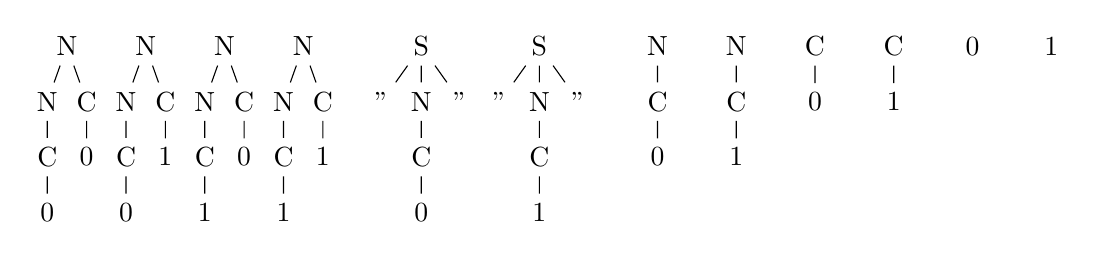
\begin{tikzpicture}[level distance=20pt]
    \tikzstyle{level 1}=[sibling distance=5mm]
\draw (0,0) node {N}
child {
    node {N}
    child {
        node {C}
        child {
            node {0}
        }
    }
}
child {
    node {C}
    child {
        node {0}
    }
};

\draw (1,0) node {N}
child {
    node {N}
    child {
        node {C}
        child {
            node {0}
        }
    }
}
child {
    node {C}
    child {
        node {1}
    }
};

\draw (2,0) node {N}
child {
    node {N}
    child {
        node {C}
        child {
            node {1}
        }
    }
}
child {
    node {C}
    child {
        node {0}
    }
};

\draw (3,0) node {N}
child {
    node {N}
    child {
        node {C}
        child {
            node {1}
        }
    }
}
child {
    node {C}
    child {
        node {1}
    }
};

\draw (4.5,0) node {S}
child {
    node {"}
}
child {
    node {N}
    child {
        node {C}
        child {
            node {0}
        }
    }
}
child {
    node {"}
};

\draw (6,0) node {S}
child {
    node {"}
}
child {
    node {N}
    child {
        node {C}
        child {
            node {1}
        }
    }
}
child {
    node {"}
};

\draw (7.5,0) node {N}
child {
    node {C}
    child {
        node {0}
    }
};

\draw (8.5,0) node {N}
child {
    node {C}
    child {
        node {1}
    }
};

\draw (9.5,0) node {C}
child {
    node {0}
};

\draw (10.5,0) node {C}
child {
    node {1}
};

\draw (11.5,0) node {0};

\draw (12.5,0) node {1};
    ;
\end{tikzpicture}
    

On prouve par induction simple qu'à l'étape $k$, on a généré tous les arbres de dérivations possibles de profondeur $\leq k$.

\subsection{La méthode top-down}

On part de l'axiome $S$ de la grammaire non contextuelle pour construire des mots de $\delta(S)$ en remplaçant un nonterminal $x$ d'un mot par un $b$ d'une règle de dérivation $(x,b)$.

Cette méthode suit d'assez près la définition des mots de la grammaire non contextuelle\\
On génère en effet, avec cette méthode, à la $n$-ième étape, 

$A_n = \left\{m \in \Sigma^\star \mid  S \left(\bigcup_{k \in [1,n]} \rightarrow^k\right) m\right\}$\\
Il est alors simple de vérifier que tout mot du langage de la grammaire sera généré en temps fini par cette méthode.

On génère alors dans l'ordre :\\
à l'étape 0 : $\{S\}$, \\
à l'étape 1 : $\{S,SS+,SS*,"N"\}$,\\
et à l'étape 2 : $\{S,SS+,SS*,"N",SS*S+,SSS*+,SSS+*,SS+S*,$ \\
$"N"S+,S"N"+,"N"S*,S"N"*,"C","NC"\}$.

Cette méthode est bien plus proche de la définition et est directement applicable aux grammaire formelles.

\section{Vérification de preuve - grammaire formelle}

\subsection{Une nouvelle structure de données pour les preuves}

Nous ne disposons plus des forêts de dérivation. Alors nous pouvons nous restreindre à la définition d'un mot qui dérive d'un autre.
On va alors fournir, comme preuve, une liste de mots $m_1, \dots, m_n$ tels que $\forall i\in [1,n-1], m_i \rightarrow m_{i+1}$. 
Pour ceci nous allons renseigner de quelle manière le mot $m_{i+1}$ dérive du mot $m_i$ par la règle de dérivation $(a,b)$, par exemple en fournissant les indices délimitant $a$ dans $m_i$, et $b$ le remplaçant.
Nous aboutissons alors à :
{\color{DarkBlue}\begin{verbatim}
type 'e preuveformelle = (int*int*('e caractere list)) list
\end{verbatim}}

Nous prendrons comme exemple la grammaire formelle $G = (T,N_t,S,D)$ où :\\
$
T = \{\underline{ a },\underline{ b },\underline{ c }\}\\
N_t = \{\underline{ S },\underline{ B }\}\\
D = \{(\underline{ S },\underline{ aBSc })_1,(\underline{ S },\underline{ abc })_2,(\underline{ Ba },\underline{ aB })_3,(\underline{ Bb },\underline{ bb })_4\}
$,\\
alors \underline{ aabbcc } est dans $\mathcal{L}(G)$ car $\underline{ S } \rightarrow_1 \underline{ aBSc } \rightarrow_2 \underline{ aBabcc } \rightarrow_3 \underline{ aaBbcc } \rightarrow_4 \underline{ aabbcc }$.\\
En Ocaml :
{\color{DarkBlue}\begin{verbatim}
let unepreuve = [(0,1,mot "aBSc");(2,3,mot "abc");(1,3,mot "aB");(2,4,mot "bb")]
\end{verbatim}}

\subsection{Vérifier une preuve dans une telle structure de données}

{\color{DarkBlue}\begin{verbatim}
let verif_deriv p grf mot = 
    let i,j,m = p in
    let achanger = soustrait i j mot in
    List.mem (aechanger,m) grf.reglesf

let verif_preuve p grf = 
    let rec aux p mot = 
        match p with
            |[] -> true
            |t::q -> 
                let i,j,m = t in
                (verif_deriv t grf) && (aux q (remplace i j mot))
    in 
    aux p [grf.axiome]

\end{verbatim}}

\section{Preuve automatique - grammaire formelle}

Chercher automatiquement une preuve d'appartenance d'un mot à une grammaire non contextuelle se fait déjà très bien avec les automates à pile.
Nous allons ici nous intéresser plus spécifiquement aux grammaires formelles, et réutiliser notre méthode top-down.
La méthode s'applique alors directement de la même manière.
Nous avons donc un algorithme qui permet théoriquement de prouver que n'importe quel mot de la grammaire appartient bien à cette dernière.
Le problème étant la complexité de ce dernier, qui fonctionne comme une machine non déterministe où on ne coupe pas les instances arrivant à un état puit.
La suite va donc consister à trouver, de manière heuristique ou non, des méthodes affirmant qu'à partir d'un mot $m$, on aura des difficultés à dériver en notre mot $m'$ à prouver.
Alors, nous allons arrêter les recherches de dérivations de S en $m'$ qui passent par le mot $m$.

Pour ce faire, pour dériver un mot $m$ en mot $m'$, on calcule $S(x) := \{x \in \Sigma^\star \mid m \rightarrow x\} 
=\{ubv \in \Sigma^\star \mid \exists (a,b) \in D / \exists (u,v)\in \Sigma^\star / x = uav\}$,
puis, pour chaque $ y \in S(x)$, on cherche une dérivation de $y$ en $m'$.

Pour calculer $S(x)$, il suffit de faire une recherche de facteur.

D'où une implémentation en OCaml : 

{\color{gray} NB :  \texttt{ remplace x i l b } donnera le mot \texttt{ x } où $x_{[i,i+l[}$ est remplacé par \texttt{ b }.

\texttt{ ppregles } est l'ensemble des règles de dérivation de la grammaire qui 
sont prétraitées pour l'algorithme kmp.\texttt{ ppregles } est donné par \texttt{ preprocessgf grf }}\\
{\color{DarkBlue}\begin{verbatim}
let preprocessgf grf =
  Array.map 
  (fun (a,b) ->
    (a,b,kmppreprocess a) 
  )
  grf.reglesf 

let succ ppregles x = 
  let res =
  List.flatten
  (
    Array.to_list (
      Array.map
      (fun (a,b,pp) ->
        List.map 
        (fun i ->
          remplace x i (Array.length a) b
        )
        (kmp x a pp)
      )
      ppregles
    )
  )
  in
  ajouteplein res []
\end{verbatim}}

\texttt{ succ ppregles x } calcule $S(x)$.

\subsection{Un parcours en largeur particulier}
Nous allons utiliser un parcours qui nous permettra de trouver dans un graphe un chemin plus court entre un sommet donné et un sommet 'valide'.
Ce parcours pourra aussi éviter les chemins passant par un sommet 'invalide'.

Alors on fournira à ce parcours une fonction \texttt{ elimine } et une fonction \texttt{ termine } toutes deux de type \texttt{ sommet -> bool }.

Ce parcours est donc un parcours en largeur depuis un sommet $x_0$ qui garde en mémoire le chemin parcouru et qui s'arrête dès qu'un 
sommet $s$, tel que \texttt{ termine s }, est parcouru. Il renvoit alors un chemin de $x_0$ à $s$. Lorsque le parcours passe par un sommet $s$ tel que \texttt{ elimine s }, 
il ne parcourt pas ensuite ses voisins.

En voici une implémentation OCaml :

{\color{DarkBlue}\begin{verbatim}
let rec parcoursmagique delta elimine termine dejavu avoir =
  let navoir = ref [] in
  let ndejavu = ref dejavu in
  if avoir = [] then None else (
  let res = 
    List.find_opt
    (function
      |[] -> failwith "mauvais chemin"
      |s::q ->
        ndejavu := ajoute s (!ndejavu);
        if (termine s) then true else
        if (elimine s || List.mem s dejavu) then false else
        (
        navoir := 
          ajouteplein
          (
            List.map
            (fun v -> v::s::q)
            (delta s)
          )
          (!navoir);
        false)
    )
    avoir
    in
  match res with
    |None -> parcoursmagique delta elimine termine (!ndejavu) (!navoir)
    |Some x -> Some x
  )
\end{verbatim}}

\subsection{Enfin, un prouveur automatique d'appartenance d'un mot à une grammaire formelle}

Il ne nous reste plus qu'à appliquer notre parcours sur un graphe où les sommets sont les mots de $\Sigma^\star$, et les
arêtes sont $\{(a,b) \in  \Sigma^\star \mid a \rightarrow b\} = \{(a,b) \in \Sigma^\star \mid b \in S(a)\}$.

En OCaml : 
{\color{DarkBlue}\begin{verbatim}
let chercherderivationnaif x m ppregles = 
  parcoursmagique
  (succ ppregles)
  (fun x -> false)
  (fun x -> x = m)
  []
  [[x]]
\end{verbatim}}

Par la suite, nous allons apporter des améliorations, en fournissant des fonctions \texttt{ elimine }.

\section{Amélioration pour les grammaires croissantes}

Une grammaire croissante est une grammaire telle que :
\begin{equation}\forall (a,b) \in D, \norm{a} \leq \norm{b} \end{equation}
On a alors une première propriété très simple, $\forall m, m' \in \delta (S), m \overset{*}{\rightarrow} m' \implies \norm{m} \leq \norm{m'}$.

Alors, dans la recherche de dérivations de S vers m, on peut supprimer les "branches de recherche" qui partent d'un mot de longueur $> \norm{m}$.
Il ne reste qu'à faire le même parcours que précédement avec la fonction suivante comme fonction \texttt{ elimine }.
{\color{DarkBlue}\begin{verbatim}
let eliminecroiss x = Array.length x > Array.length m
\end{verbatim}}

\section{Amélioration dans le cas général : déduction sur le nombre d'occurence de chaque lettre}
Rappelons, le problème : étant donné un mot $m$ d'une grammaire, comment le dériver en un mot $m'$ ?
Pour tout $l \in \Sigma$, on va chercher un ensemble $q(l)$ qui majore $\norm{\delta(m)}_l$ ($=\{\norm{x}_l \mid x \in \delta(m)\}$).

Ainsi, $m \overset{*}{\rightarrow} m' \implies \norm{m'}_l \in q(l)$, la contraposée nous sera utile : 
\begin{equation*}
\norm{m'}_l \notin q(l) \implies  \neg (m \overset{*}{\rightarrow} m')
\end{equation*}
Ce qui pourra nous permettre de réduire notre champ de recherche.
En effet, 

\fbox{si pour un mot $x \in \delta(m)$, $\forall l \in \Sigma, \norm{\delta(x)}_l \cap q(l) = \emptyset$,
 alors $m' \notin \delta(x)$}.

Pour calculer $\norm{\delta(x)}_l \cap q(l)$, nous allons utiliser un graphe semblable à un automate.

Les sommets sont des états de $Q \subset ({\mathcal{P}(\mathbb{N})})^{\Sigma}$ tels que :
\begin{align*}
    &\forall q,q' \in Q, \exists l \in \Sigma / q(l) \cap q'(l) = \emptyset\\
    \text{ et }&\forall m \in \delta(S), \exists q \in Q / \forall l \in \Sigma, \norm{m}_l \in q(l)
\end{align*}

Ainsi à tout mot $x \in \delta(S)$, on peut associer un unique état $q$ tel que $\forall l \in \Sigma, \norm{x}_l \in q(l)$, notons cet état $cat(x)$

Les arêtes du graphe sont les dérivation possibles d'un famille majorante $q$ à une autre $q'$.
\begin{equation*}
    \forall (q,q') \in Q^2, (q,q') \in A \iff \exists x,x' \in \Sigma^\star / x \rightarrow x' \text{ et } \forall l \in \Sigma, \norm{x}_l \in q(l) \text{ et } \norm{x'}_l \in q(l)
\end{equation*}

Ainsi, si $m$ correspond à un état $q$, et $m'$ à un état $q'$, alors $m \overset{*}{\rightarrow} m' \implies$ $q'$ est accessible depuis $q$.

\subsection{Les états $q$ sous la forme $q \in Q = \{\{0\},\mathbb{N}^*\}^{\Sigma}$}
Exemple avec la grammaire suivante :
$D := \{(S,\underline{ abc })_0,(\underline{ abc },\underline{ ab })_1,(\underline{ b },\underline{ k })_2,(\underline{ c },\underline{ ak })_3,(\underline{ kak },\underline{ aa })_4,(\underline{ a },\underline{ aaa })_5\}$

Le graphe est le suivant :

 \tikzfig{grosgraphe}

Et voici ce à quoi correspondent les différents états (sommets) du graphe : 

 
\begin{table}[!h]
\begin{tabular}{|l| |l|l|l|l|l|l|l|l|l|}
\hline
$q$    & $\alpha$ & $\beta$ & $\gamma$ & $\delta$ & $\epsilon$ & $\varphi$ & $\psi$ & $\mu$ & $\sigma$ \\ \hline \hline
$q(a)$ & $\mathbb{N}^*$        & $\mathbb{N}^*$       & $\mathbb{N}^*$        & $\mathbb{N}^*$        & $\mathbb{N}^*$          & $\mathbb{N}^*$         & $\mathbb{N}^*$      & $\mathbb{N}^*$     & $\{0\}$        \\ \hline
$q(b)$ & $\mathbb{N}^*$        & $\mathbb{N}^*$       & $\{0\}$        & $\mathbb{N}^*$        & $\{0\}$          & $\{0\}$         & $\{0\}$      & $\mathbb{N}^*$     & $\{0\}$        \\ \hline
$q(c)$ & $\mathbb{N}^*$        & $\{0\}$       & $\mathbb{N}^*$        & $\{0\}$        & $\{0\}$          & $\{0\}$         & $\mathbb{N}^*$      & $\mathbb{N}^*$     & $\{0\}$        \\ \hline
$q(k)$ & $\{0\}$        & $\{0\}$       & $\{0\}$        & $\mathbb{N}^*$        & $\mathbb{N}^*$          & $\{0\}$         & $\mathbb{N}^*$      & $\mathbb{N}^*$     & $\{0\}$        \\ \hline
$q(S)$ & $\{0\}$        & $\{0\}$       & $\{0\}$        & $\{0\}$        & $\{0\}$          & $\{0\}$         & $\{0\}$      & $\{0\}$     & $\mathbb{N}^*$        \\ \hline
\end{tabular}
\end{table}

Le graphe réduit suivant sera utile : 

 \tikzfig{ptitgraphe}

Ainsi, nous pouvons tout de suite affirmer qu'il est impossible de dériver \underline{ aaabakab } en \underline{ akkcckaaakck } (en effet, $\psi$ n'est pas accessible depuis $\delta$)

Intéressons nous au calcul des arrêtes $A$ du graphe.

Considérons d'abord les arêtes partant d'un état $q$ donné, puis celles correspondant à une dérivation $d$ donnée.

$A_q(\Sigma) := \{(a,b) \in A \mid a = q\}$

$A_{q,d}(\Sigma) := \{(a,b) \in A_q \mid \exists x,x' \in \Sigma^\star / x \overset{d}{\rightarrow} x' \text{ et } cat(x) = q \text{ et } cat(x') = q'\}$

Soit $l \in \Sigma$,

\begin{answer} 
$\Sigma ' := \Sigma \backslash \{l\}$

On a alors $A_q(\Sigma) = \bigcup_{d \in D} A_{q,d}(\Sigma)$ et $A = \bigcup_{q \in Q} A_q(\Sigma)$.

Et les $A_{q,d}(\Sigma)$ sont majorables de la manière suivante : 


Si $cat(b)(l) = \mathbb{N}^\star$, alors
\begin{answer} 
\begin{equation*}A_{q,d}(\Sigma) \subset \{(q,b) \in Q^2 \mid (q_{\Sigma '},b_{\Sigma '}) \in A_{q,d}(\Sigma ') \text{ et } b(l) = \mathbb{N}^\star\}\end{equation*}
En effet, si $d$ produit la lettre $l$, elle est forcément dans le mot produit.
\end{answer}


Si $cat(b)(l) = \{0\}$ et $q(l) = \{0\}$, alors 
\begin{answer} 
\begin{equation*}A_{q,d}(\Sigma) \subset \{(q,b) \in Q^2 \mid (q_{\Sigma '},b_{\Sigma '}) \in A_{q,d}(\Sigma ') \text{ et } b(l) = \{0\}\}\end{equation*}
En effet, si $x$ ne contient pas la lettre $l$, et que $d$ ne produit pas la lettre $l$, le mot produit $x'$ n'aura pas de $l$.
\end{answer}


Si $cat(b)(l) = \{0\}$ et $q(l) = \Sigma^\star$, alors
\begin{answer} 
\begin{align*}
A_{q,d}(\Sigma) \subset &\{(q,b) \in Q^2 \mid (q_{\Sigma '},b_{\Sigma '}) \in A_{q,d}(\Sigma ') \text{ et } b(l) = \{0\}\} \\
\cup &\{(q,b) \in Q^2 \mid (q_{\Sigma '},b_{\Sigma '}) \in A_{q,d}(\Sigma ') \text{ et } b(l) = \Sigma^\star\}
\end{align*}
On ne peut rien dire, alors les deux prolongements possibles (sur la valeur de $b(l)$) seront explorés.
\end{answer}
\end{answer}

On peut alors majorer l'ensemble des arêtes du graphe.

Maintenant, une fois le graphe majorant associé à notre grammaire calculé, on peut faire notre fonction \texttt{ elimine },
 \texttt{ elimine x } renvoit vrai si et seulement si $x$ n'est pas accessible depuis S dans le graphe majorant.
 (On peut précalculer le graphe réduit où les sommets sont les composantes fortement connexes et sa matrice
 d'accessibilité avec l'algorithme Floyd Warshall par exemple, pour réduire les temps de calcul).

\end{document}
    